\documentclass{beamer}
\mode<presentation>
{
  \usetheme{default}
  \usecolortheme{default} 
  \usefonttheme{default} 
  \setbeamertemplate{navigation symbols}{}
  \setbeamertemplate{caption}[numbered]
  \setbeamercolor{title}{fg=white}
  \setbeamercolor{author}{fg=gray}
  \setbeamercolor{institute}{fg=gray}
} 

\usepackage[english]{babel}
\usepackage[utf8x]{inputenc}
\usepackage{color}
\usepackage{amsmath}
\usepackage{amssymb}
\usepackage{graphics}

\title[Time is on your side]{Time is on your side: \\
Semantic enrichment of time series}
\author{Bojan Bo\v{z}i\'{c}}
\institute{Dublin Institute of Technology}
\date{}

\begin{document}
{\usebackgroundtemplate{
\includegraphics[width=\paperwidth,height=\paperheight]{cover.jpg}}
\begin{frame}
  \titlepage
\end{frame}}

\section{Time Series Analysis}

\begin{frame}{What is a time series?}
\begin{itemize}
  \item What we need: value(s) + time stamp
  \item What would be grand: constant time interval
  \item Mathematically: values $Y_1, Y_2, ...$ of a variable $Y$ at points in time $t_1, t_2, ...$ Therefore: $Y = F(t)$
\end{itemize}
\vskip 1cm
\begin{block}{Example}
Air quality sensor measuring carbon monoxide and ozone concentrations in air (in ppm), and sending in values every 10 minutes.
\end{block}
\end{frame}

\begin{frame}{Subdisciplines and Goals}
We distinguish:
\begin{itemize}
\item Time Series Analysis: Analysing time series data in order to extract meaningful statistics and other characteristics of the data.
\item Time Series Forecasting: Estimating many future aspects of a business or other operation based on the current time series.
\end{itemize}
Which aim at:
\begin{itemize}
\item Identifying the nature of the phenomenon represented by the sequences of operations.
\item Predicting future values of the time series variables.
\end{itemize}
\end{frame}


{\usebackgroundtemplate{
\includegraphics[width=\paperwidth,height=\paperheight]{patterns.jpg}}
\begin{frame}{\textcolor{white}{Patterns}}
\centering
\begin{tabular}{ll}
\colorbox{white}{Trend:} %long term direction
& \colorbox{white}{Seasonal:} \\ %regular pattern within time periods
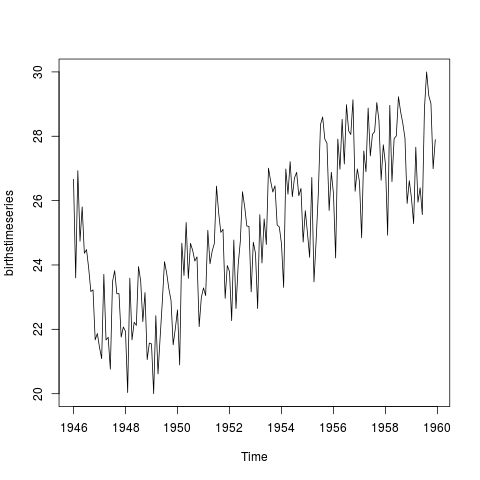
\includegraphics[width=3.5cm]{birthstimeseries} & 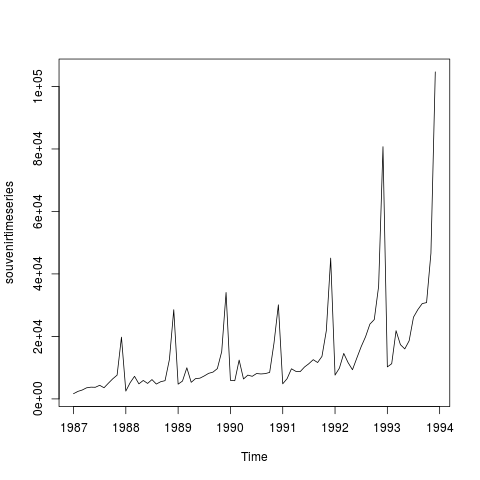
\includegraphics[width=3.5cm]{souvenirtimeseries} \\ %occurs regularly but may vary in length
\colorbox{white}{Cyclical:} & \colorbox{white}{Irregular:} \\ 
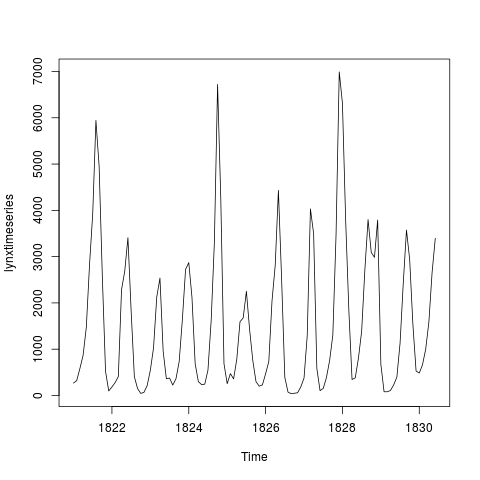
\includegraphics[width=3.5cm]{lynxtimeseries} & 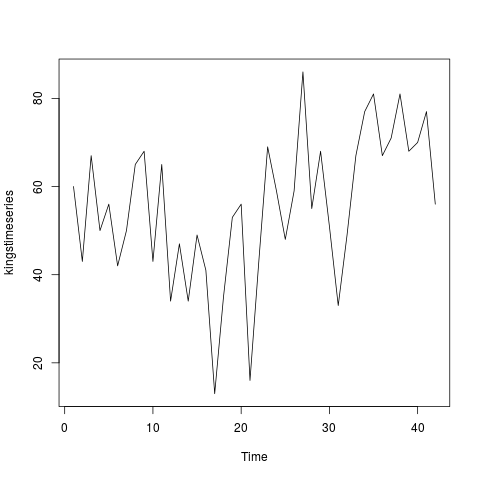
\includegraphics[width=3.5cm]{kingstimeseries} \\ %unpredictable, random fluctuations
\end{tabular}
\end{frame}}

\begin{frame}{Decomposition}
\begin{figure}
\centering
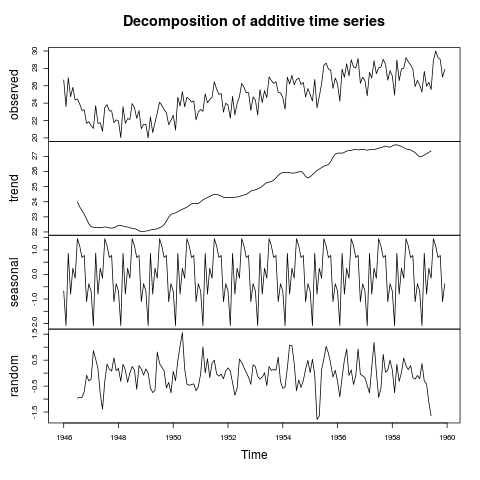
\includegraphics[width=7cm]{birthstimeseriescomponents}
\caption{Decomposed births time series.}
\end{figure}
\end{frame}

\begin{frame}{Mathematical Models}
Additive Model:
\begin{enumerate}
\item Assume data is sum of components: $Y_t = T + S + C + I$
\item If one of the components is not contained the value is zero, therefore: $Y_t = T + S + I$
\item Seasonal component is independent of trend $\implies$ magnitude of seasonal swing is constant
\end{enumerate}
Multiplicative Model:
\begin{enumerate}
\item Assume data is product of components: $Y_t = T * S * C * I$
\item If one of the components is missing, the value is assumed to be 1: $Y_t = T * S * I$
\item Seasonal factor is a ratio to the trend $\implies$ magnitude increases or decreases according to trend
\end{enumerate}
\end{frame}

\begin{frame}{Smoothing}
\begin{itemize}
\item Removes random variation and shows trends and cycles
\item Two methods:
\begin{enumerate}
\item Averaging Smoothing: e.g. $SMA_i = \frac{\sum_{k=i-n}^{i}x_k}{n}$
\item Exponential Smoothing: e.g. $EMA_i = EMA_{i-1} + \alpha * (x_i - EMA_{i-1})$ \\ $\alpha = \frac{2}{n+1} $
%larger weights to more recent observations
\end{enumerate}
\end{itemize}
\begin{figure}
\centering
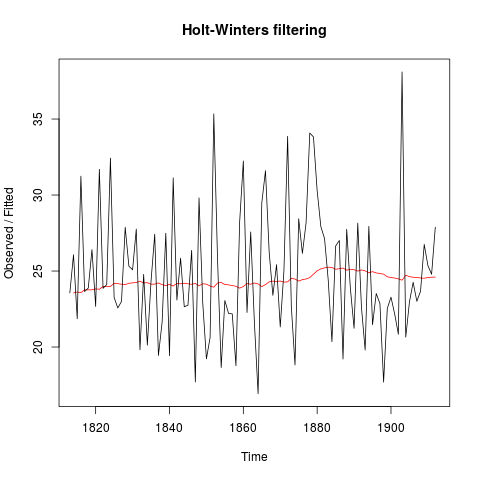
\includegraphics[width=4cm]{holt-winters}
\caption{Smoothed forecasts for rainfall using Holt-Winters (Simple Exponential Smoothing)}
\end{figure}
\end{frame}

\section{Semantic Time Series}
\begin{frame}{Why add Semantics?}
\begin{itemize}
\item Experts in different fields have to deal with time series (environment,
finance, etc.)
\item Time series represent measurements with a lot of data (values for
years with measurements for every second)
\item A lot of time and expert knowledge required to find the right part of a
time series
\item Time series processors are highly customized and developed
exclusively for one purpose
\end{itemize}
\end{frame}

\begin{frame}{Expressions}
\begin{table}                                                             
\centering                                                                
\begin{tabular}{|l|l|}                                                    
\hline                                                                    
\textbf{Expression} & \textbf{Meaning} \\                                 
\hline                                                                    
\texttt{< [n].sin * 2 + 3 >} & Calculation is applied to all slots. \\    
\hline                                                                    
\texttt{A, B < A[n] + 2 * B[n] >} & Combination of two time series \\     
& (aggregation). \\                                                       
\hline                                                                    
\texttt{< [n] > every 2 hours} & Projection to a fixed time grid. \\      
\hline                                                                    
\texttt{< (t .. t-2).mean >} & Sliding mean value. \\                     
\texttt{every 1 hour} & \\                                                
\hline                                                                    
\texttt{< [n]->hot if} & Filtering, classification. \\                    
\texttt{[n].temperature > 100} & \\                                       
\texttt{otherwise [n]->cold >} & \\                                       
\hline                                                                    
\end{tabular}  
\caption{An overview of most commonly used time series processing expressions.}
\end{table}
\end{frame}

\begin{frame}{Semantic Time Series}
\begin{itemize}
\item Enrichment of time series with meta-information (annotations)
\item Reduction of processor and language complexity
\item Usage of ontologies to define the domain of interest
\item Usage of reasoning to generate new meta-information
\end{itemize}
\end{frame}

\begin{frame}{Comparison}
\begin{figure}
\centering
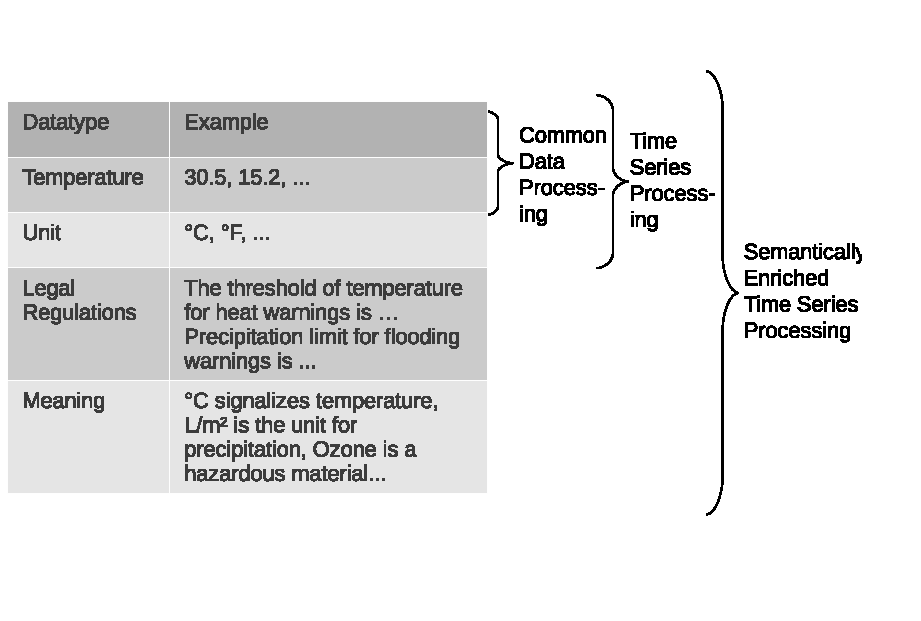
\includegraphics[width=10cm]{semantic-ts-eps-converted-to}
\caption{Difference between one-dimensional data, time series, and semantic time series}
\end{figure}
\end{frame}

\begin{frame}{Sample Semantic Expression}
Sample regular Time Series Processing expression:\\                       
\texttt{MeteoTS < warning if precipitation > 1000 l/m$^2$ or}\\           
\texttt{temperature > 40$^\circ$C or wind > 56 knots ... >}\\             
\vspace{15pt}                                                             
Semantic Time Series Processing expression:\\                             
\texttt{MeteoTS < warning if value > allowed >} 
\end{frame}

\begin{frame}{Ontologies}
\begin{enumerate}
\item Definition of all common classes and properties, which are valid for all
possible time series ontologies.
\item Extraction of a bridge ontology which can be used as a common
interface for all domain ontologies.
\item Every individual domain ontology needs to inherit from the bridge
ontology (it has to define all classes which are also defined in the
bridge ontology).
\item Therefore, an ontology graph can be constructed, which has the
bridge ontology in the center.
\end{enumerate}
\end{frame}

\begin{frame}{Time Series Ontology}
\begin{figure}
\centering
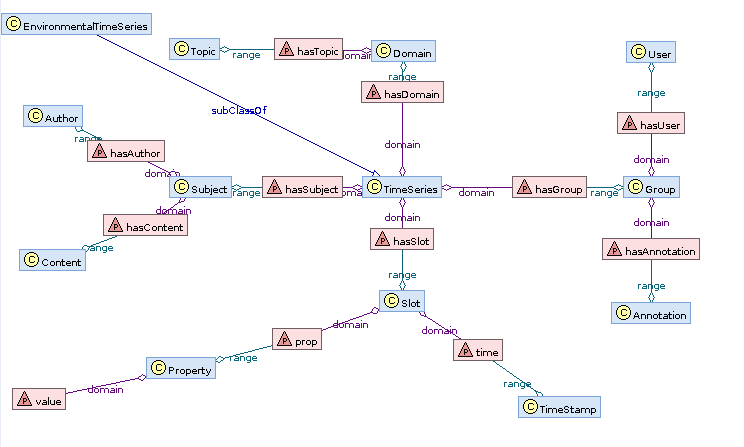
\includegraphics[width=10cm]{bridge}
\caption{The Time Series Bridge Ontology for connecting domain knowledge.}
\end{figure}
\end{frame}

\begin{frame}{Contact}

\includegraphics[width=10cm]{ceadar} 
\begin{flushleft}
Bojan Bo\v{z}i\'{c} \\
CeADAR Research Fellow \\
Email: bojan.bozic@dit.ie \\
Twitter: @bojan\_bozic 
\end{flushleft}
\begin{flushleft}
TimeSeries data: robjhyndman.com/tsdldata/ \\
Images: suwalls.com, patterncooler.com
\end{flushleft}
\end{frame}

% In this booklet, I will be using time series data sets that have been kindly made available by Rob Hyndman in his Time Series Data Library at http://robjhyndman.com/TSDL/.
\end{document}
